\chapter{Appendix}\label{chap:appendix}
% \begin{appendices}

\section{Github Repository}\label{github}

We are on Github! (\url{https://github.com/la-mar/Applied-Stats-Project-2})

All code used in our analysis is included in the appendix below, but we recommend viewing it in its original form in our github repository.

\section{Appendix A}\label{appendix-a}



\subsection{Model Comparison - Continued}\label{moremodelcomp}

\begin{figure}[!hb]
    \center{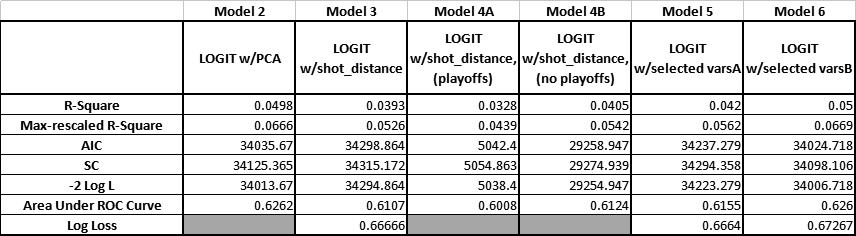
\includegraphics[width=\textwidth]{../figs/modelcomparison.png}}
    % \caption{\label{fig:ldaresults} SAS: LDA Results}
\end{figure}

\begin{figure}[!hb]
    \center{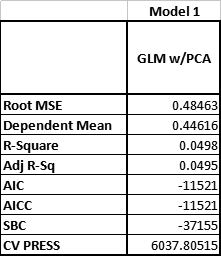
\includegraphics[width=\textwidth]{../figs/glm_pca.png}}
    % \caption{\label{fig:plotproba} Predicted Shot Probability over Distance to Hoop}
\end{figure}

\begin{figure}[!hb]
    \center{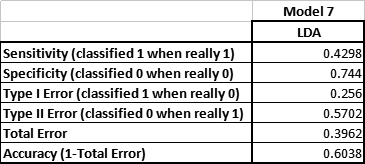
\includegraphics[width=\textwidth]{../figs/lda.png}}
    % \caption{\label{fig:plotproba} Predicted Shot Probability over Distance to Hoop}
\end{figure}


\subsection{Data Dictionary}\label{datadictionary}
\resizebox{\textwidth}{!}{
\begin{table}[h]
    \centering
    \begin{tabular}{llllllllllllllll}
    Alphabetic & List & of & Variables & and & Attributes &  &  &  &  &  &  &  &  &  &  \\
    \#	Variable	Type	Format	Description &  &  &  &  &  &  &  &  &  &  &  &  &  &  &  \\
    2	action\_type	Char	17	The & type & of & shot & that & was & attempted & (e.g. & Jump Shot, & Driving Dunk) &  &  &  &  &  &  \\
    28	arena\_temp	Num	BEST12.	The & average & temperature & in & the & arena & during & the & game &  &  &  &  &  &  &  \\
    27	attendance	Num	BEST12.	The & number & of & people & attending & the & game &  &  &  &  &  &  &  &  &  \\
    29	avgnoisedb	Num	BEST12.	The & average & noise & (in & decibels) & during & the & game &  &  &  &  &  &  &  &  \\
    3	combined\_shot\_type	Char	9	The & type & of & combined & shot & that & was & attempted & (e.g. & Jump Shot, & Dunk) &  &  &  &  &  \\
    23	game\_date	Num	MMDDYY10.	The & date & that & the & game & occurred & on &  &  &  &  &  &  &  &  &  \\
    4	game\_event\_id	Num	BEST12.	The & id & of & the & specific & event & associated & with & this & shot & attempt &  &  &  &  &  \\
    5	game\_id	Num	BEST12.	The & id & of & the & specific & game &  &  &  &  &  &  &  &  &  &  \\
    6	lat	Num	BEST12.	The & location & (in & latitude) & of & the & shot & attempt &  &  &  &  &  &  &  &  \\
    7	loc\_x	Num	BEST12.	The & x & coordinate & of & the & shot & attempt & (based & on & the & x & y & grid & of & the & court) \\
    8	loc\_y	Num	BEST12.	The & y & coordinate & of & the & shot & attempt & (based & on & the & x & y & grid & of & the & court) \\
    9	lon	Num	BEST12.	The & location & (in & longitude) & of & the & shot & attempt &  &  &  &  &  &  &  &  \\
    24	matchup	Char	11	The & matchup & of & the & two & teams & playing & (e.g. & LAL @ POR) &  &  &  &  &  &  &  \\
    10	minutes\_remaining	Num	BEST12.	The & number & of & minutes & remaining & in & the & period & in & which & the & shot & attempt & occurred &  &  \\
    25	opponent	Char	3	The & NBA & abbreviation & of & the & opposing & team &  &  &  &  &  &  &  &  &  \\
    11	period	Num	BEST12.	The & period & of & the & game & in & which & the & shot & attempt & occurred &  &  &  &  &  \\
    12	playoffs	Num	BEST12.	Whether & or & not & the & game & was & a & playoff & game &  &  &  &  &  &  &  \\
    1	recId	Num	BEST12.	The & unique & id & of & the & observation & of & the & shot & attempt & (in & chronological & order) &  &  &  \\
    13	season	Num	YYYYYY	The & YearYr & indicator & of & the & game & season & (e.g. & 200001 & = & 2000-2001 & season) &  &  &  &  \\
    14	seconds\_remaining	Num	BEST12.	The & number & of & seconds & remaining & in & the & period & (concatenated & with & associated & minutes) &  &  &  &  \\
    in & which & the & shot & attempt & occurred &  &  &  &  &  &  &  &  &  &  \\
    15	shot\_distance	Num	BEST12.	The & distance & of & the & shot & attempt & (in & feet) &  &  &  &  &  &  &  &  \\
    26	shot\_id	Num	BEST12.	The & id & of & the & specific & shot & attempt & within & the & game &  &  &  &  &  &  \\
    16	shot\_made\_flag	Num	BEST12.	Whether & or & not & the & shot & attempt & resulted & in & a & successful & shot &  &  &  &  &  \\
    17	shot\_type	Char	14	The & technical & term & for & the & type & of & shot & that & was & attempted & (e.g. & 2PT Field Goal) &  &  &  \\
    18	shot\_zone\_area	Char	21	The & zone & location & on & the & court & that & the & shot & attempt & occurred & ("Left & Side(L)", & Center(C)) &  &  \\
    19	shot\_zone\_basic	Char	21	The & approximate & zone & location & on & the & court & that & the & shot & attempt & occurred & ("Mid & Range", &  &  \\
    Restricted Area) &  &  &  &  &  &  &  &  &  &  &  &  &  &  &  \\
    20	shot\_zone\_range	Char	15	The & distance & range & in & feet & of & the & zone & location & to & the & goal & ("8-16 & ft.", & 16-24 ft.) &  \\
    21	team\_id	Num	BEST12.	NBA & league & team & id &  &  &  &  &  &  &  &  &  &  &  &  \\
    22	team\_name	Char	18	NBA & league & team & name &  &  &  &  &  &  &  &  &  &  &  &
    \end{tabular}
    \end{table}
}
\section{SAS Code}\label{sascode}
\begin{minted}[mathescape,
    linenos,
    numbersep=5pt,
    gobble=2,
    frame=lines,
    framesep=2mm,
    breaklines]{SAS}
/* MSDS 6371 - Applied Statistics  */
/* Allen Crane and Brock Friedrich */
/* Kobe Bryant Shot Selection      */
/* November 2018                   */

/* import data */
proc import datafile="c:\users\allen\documents\smu data science\MSDS 6372 - Applied Statistics\project 2\project2Data.csv"
          dbms=dlm out=train replace;
     delimiter=',';
     getnames=yes;
run;

/* print data */
proc print data=train (obs=10);
run;

/* investigate data for variable types*/
proc contents data=train;
run;

/* look for missing numeric data - may need to impute */
proc means data = train n nmiss;
  var _numeric_;
run;

/* investigate means of training data and any missing values */
proc means data = train n nmiss;
run;

/* univariate data analysis */
proc univariate data = train;
var season;
run;

/* note that certain "season" fields are missing */
Data _season;
    set train;
    where missing (season);
run;

/* print "season" data, where "season" is missing */
proc print data=_season (obs=200);
run;


/* more univariate data analysis */
ods graphics on;
proc univariate data = train plot;
var recId
game_event_id
game_id
lat
loc_x
loc_y
lon
minutes_remaining
period
playoffs
season
seconds_remaining
shot_distance
shot_made_flag
team_id
game_date
shot_id
attendance
arena_temp
avgnoisedb
;
run;
ods graphics off;

/* create a time-based variable, concatenating Period, minutes remaining, and seconds remaining, in descending order. This one is for Periods remaining... */
data train2;
  set train;
      if period = 1 then periods_remaining2 = "14";
      else if period = 2 then periods_remaining2 = "28";
	  else if period = 3 then periods_remaining2 = "42";
	  else if period = 4 then periods_remaining2 = "57";
	  else if period = 5 then periods_remaining2 = "71";
	  else if period = 6 then periods_remaining2 = "85";
	  else if period = 7 then periods_remaining2 = "99";
	  else periods_remaining2 = period;
run;

/* print data */
proc print data=train2 (obs=10);
run;

/* Minutes remaining... */
data train2;
  set train2;
      if minutes_remaining = 11 then minutes_remaining2 = "99";
      else if minutes_remaining = 10 then minutes_remaining2 = "90";
	  else if minutes_remaining = 9 then minutes_remaining2 = "81";
	  else if minutes_remaining = 8 then minutes_remaining2 = "72";
	  else if minutes_remaining = 7 then minutes_remaining2 = "63";
	  else if minutes_remaining = 6 then minutes_remaining2 = "54";
	  else if minutes_remaining = 5 then minutes_remaining2 = "45";
	  else if minutes_remaining = 4 then minutes_remaining2 = "36";
	  else if minutes_remaining = 3 then minutes_remaining2 = "27";
	  else if minutes_remaining = 2 then minutes_remaining2 = "18";
	  else if minutes_remaining = 1 then minutes_remaining2 = "09";
	  else if minutes_remaining = 0 then minutes_remaining2 = "00";
	  else minutes_remaining2 = minutes_remaining;
run;

/* print data */
proc print data=train2 (obs=10);
run;

/* Seconds remaining... */
data train2;
  set train2;
      if seconds_remaining = 59 then seconds_remaining2 = "99";
      else if seconds_remaining = 58 then seconds_remaining2 = "97.3";
	  else if seconds_remaining = 57 then seconds_remaining2 = "95.6";
	  else if seconds_remaining = 56 then seconds_remaining2 = "94";
	  else if seconds_remaining = 55 then seconds_remaining2 = "92.3";
	  else if seconds_remaining = 54 then seconds_remaining2 = "90.6";
	  else if seconds_remaining = 53 then seconds_remaining2 = "88.9";
	  else if seconds_remaining = 52 then seconds_remaining2 = "87.3";
	  else if seconds_remaining = 51 then seconds_remaining2 = "85.6";
	  else if seconds_remaining = 50 then seconds_remaining2 = "83.9";
	  else if seconds_remaining = 49 then seconds_remaining2 = "82.2";
	  else if seconds_remaining = 48 then seconds_remaining2 = "80.5";
      else if seconds_remaining = 47 then seconds_remaining2 = "78.9";
	  else if seconds_remaining = 46 then seconds_remaining2 = "77.2";
	  else if seconds_remaining = 45 then seconds_remaining2 = "75.5";
	  else if seconds_remaining = 44 then seconds_remaining2 = "73.8";
	  else if seconds_remaining = 43 then seconds_remaining2 = "72.2";
	  else if seconds_remaining = 42 then seconds_remaining2 = "70.5";
	  else if seconds_remaining = 41 then seconds_remaining2 = "68.8";
	  else if seconds_remaining = 40 then seconds_remaining2 = "67.1";
	  else if seconds_remaining = 39 then seconds_remaining2 = "65.4";
	  else if seconds_remaining = 38 then seconds_remaining2 = "63.8";
	  else if seconds_remaining = 37 then seconds_remaining2 = "62.1";
	  else if seconds_remaining = 36 then seconds_remaining2 = "60.4";
	  else if seconds_remaining = 35 then seconds_remaining2 = "58.7";
	  else if seconds_remaining = 34 then seconds_remaining2 = "57.1";
	  else if seconds_remaining = 33 then seconds_remaining2 = "55.4";
	  else if seconds_remaining = 32 then seconds_remaining2 = "53.7";
	  else if seconds_remaining = 31 then seconds_remaining2 = "52";
	  else if seconds_remaining = 30 then seconds_remaining2 = "50.3";
	  else if seconds_remaining = 29 then seconds_remaining2 = "48.7";
      else if seconds_remaining = 28 then seconds_remaining2 = "47";
	  else if seconds_remaining = 27 then seconds_remaining2 = "45.3";
	  else if seconds_remaining = 26 then seconds_remaining2 = "43.6";
	  else if seconds_remaining = 25 then seconds_remaining2 = "41.9";
	  else if seconds_remaining = 24 then seconds_remaining2 = "40.3";
	  else if seconds_remaining = 23 then seconds_remaining2 = "38.6";
	  else if seconds_remaining = 22 then seconds_remaining2 = "36.9";
	  else if seconds_remaining = 21 then seconds_remaining2 = "35.2";
	  else if seconds_remaining = 20 then seconds_remaining2 = "33.6";
	  else if seconds_remaining = 19 then seconds_remaining2 = "31.9";
	  else if seconds_remaining = 18 then seconds_remaining2 = "30.2";
	  else if seconds_remaining = 17 then seconds_remaining2 = "28.5";
	  else if seconds_remaining = 16 then seconds_remaining2 = "26.8";
	  else if seconds_remaining = 15 then seconds_remaining2 = "25.2";
	  else if seconds_remaining = 14 then seconds_remaining2 = "23.5";
	  else if seconds_remaining = 13 then seconds_remaining2 = "21.8";
	  else if seconds_remaining = 12 then seconds_remaining2 = "20.1";
	  else if seconds_remaining = 11 then seconds_remaining2 = "18.5";
	  else if seconds_remaining = 10 then seconds_remaining2 = "16.8";
	  else if seconds_remaining = 9 then seconds_remaining2 = "15.1";
      else if seconds_remaining = 8 then seconds_remaining2 = "13.4";
	  else if seconds_remaining = 7 then seconds_remaining2 = "11.7";
	  else if seconds_remaining = 6 then seconds_remaining2 = "10.1";
	  else if seconds_remaining = 5 then seconds_remaining2 = "08.4";
	  else if seconds_remaining = 4 then seconds_remaining2 = "06.7";
	  else if seconds_remaining = 3 then seconds_remaining2 = "05";
	  else if seconds_remaining = 2 then seconds_remaining2 = "03.4";
	  else if seconds_remaining = 1 then seconds_remaining2 = "01.7";
	  else if seconds_remaining = 0 then seconds_remaining2 = "00";
else seconds_remaining2 = seconds_remaining;
run;

/* print data */
proc print data=train2 (obs=10);
run;

/* concatenante data */
data train2;
set train2;
pms_remaining = cat(periods_remaining2, minutes_remaining2, seconds_remaining2);
run;

/* print data */
proc print data=train2 (obs=10);
run;

/* make field numeric (some components contained leading zeroes */
data train2;
set train2;
   n_pms_remaining = input(pms_remaining,8.);
run;

/* drop original non-numeric concetenanted data field */
data train2;
set train2 (drop = pms_remaining);
run;
data train2;

/* rename new numeric concatenated data field  */
set train2 (rename=(
'n_pms_remaining'n='pms_remaining'n));
run;

/* print data */
proc print data=train2 (obs=10);
run;





/* check data - histogram */
ods graphics on;
proc univariate data = train2;
var pms_remaining;
histogram;
run;
ods graphics off;

/* check data - scatter plot */
proc sgplot data=train2;
   scatter x=pms_remaining y=shot_made_flag / group=shot_made_flag;
run;



/* transform data - log transformation on shot distance and time remaining */
data train3;
set train2;
l_shot_distance = log(shot_distance);
l_pms_remaining = log(pms_remaining);
run;


/* check data - scatter plot */
ods graphics on;
proc univariate data = train3 plot;
var l_shot_distance l_pms_remaining;
run;
ods graphics off;




/* correlation analysis */
ods graphics on;
proc corr data=train2 plots=matrix(histogram);
var recId
game_event_id
game_id
lat
loc_x
loc_y
lon
minutes_remaining
period
playoffs
season
seconds_remaining
shot_distance
shot_made_flag
team_id
game_date
shot_id
attendance
arena_temp
avgnoisedb;
run;
ods graphics off;



/* principal component analysis */
ods graphics on;
proc princomp plots=all data=train2 cov out=pca;
var recId
game_event_id
game_id
lat
loc_x
loc_y
lon
minutes_remaining
period
playoffs
season
seconds_remaining
shot_distance
shot_made_flag
team_id
game_date
shot_id
attendance
arena_temp
avgnoisedb;
run;
ods graphics off;


/* correlation analysis using train2 data vs shot made flag */
proc corr data=train2 plots=matrix(histogram);
      var shot_made_flag game_event_id lat loc_y minutes_remaining period seconds_remaining shot_distance attendance arena_temp avgnoisedb;
      run;


/* correlation analysis using pricipal components vs shot made flag */
proc corr data=pca plots=matrix(histogram);
      var shot_made_flag prin1 - prin10;
      run;


/* model 1 - GLM select using PCA */
proc glmselect data=pca plots=all seed=3;
model shot_made_flag =prin1-prin10 / selection = stepwise(choose=CV select=CV stop=CV);
run;


/* model 2 - Logistic using PCA */
ods graphics on;
proc logistic data=pca plots(only)=(roc(id=obs) effect);
  model shot_made_flag (event='1') =prin1-prin10 / scale=none
                            		clparm=wald
                            		clodds=pl
                            		rsquare
									lackfit
									ctable;
  output out = model_2_results p = Predict;
run;
ods graphics off;


/* model 3 - Logistic using train2 dataset (not PCA) only by distance */
ods graphics on;
proc logistic data=train2 plots(only)=(roc(id=obs) effect);
  model shot_made_flag (event='1') = shot_distance / scale=none
                            		clparm=wald
                            		clodds=pl
                            		rsquare
									lackfit
									ctable;
  output out = model_3_results p = Predict;
run;
ods graphics off;


/* create data for model 4 - data sets for playoffs and not at playoffs */

data train2_playoffs;
set train2;
where playoffs = 1;
run;

data train2_no_playoffs;
set train2;
where playoffs = 0;
run;


/* model 4A - Logistic using train2 dataset (not PCA) during playoffs */

ods graphics on;
proc logistic data=train2_playoffs plots(only)=(roc(id=obs) effect);
  model shot_made_flag (event='1') = shot_distance / scale=none
                            		clparm=wald
                            		clodds=pl
                            		rsquare
									lackfit
									ctable;
  output out = model_4A_results p = Predict;
run;
ods graphics off;


/* model 4B - Logistic using train2 dataset (not PCA) during playoffs */

ods graphics on;
proc logistic data=train2_no_playoffs plots(only)=(roc(id=obs) effect);
  model shot_made_flag (event='1') = shot_distance / scale=none
                            		clparm=wald
                            		clodds=pl
                            		rsquare
									lackfit
									ctable;
  output out = model_4B_results p = Predict;
run;
ods graphics off;


/* model 5 - Logistic using train2 dataset (not PCA) during playoffs */
ods graphics on;
proc logistic data=train2 plots(only)=(roc(id=obs) effect);
  model shot_made_flag (event='1') = shot_distance playoffs arena_temp game_event_id lat lon / scale=none
                            		clparm=wald
                            		clodds=pl
                            		rsquare
									lackfit
									ctable;
  output out = model_5_results p = Predict;
run;
ods graphics off;


/* model 6 - Logistic using train2 dataset (not PCA) for all variables that had corr p < 0.0001 */
ods graphics on;
proc logistic data=train2 plots(only)=(roc(id=obs) effect);
  model shot_made_flag (event='1') = shot_distance playoffs period minutes_remaining seconds_remaining attendance arena_temp avgnoisedb / scale=none
                            		clparm=wald
                            		clodds=pl
                            		rsquare
									lackfit
									ctable;
  output out = model_6_results p = Predict;
run;
ods graphics off;


/* Model 7 - LDA Model */

proc discrim data=train2 outstat=LDAstat method=normal pool=yes
                list crossvalidate;
      class shot_made_flag;
      priors prop;
      var shot_distance playoffs period minutes_remaining seconds_remaining attendance arena_temp avgnoisedb;
   run;









/* Import test data for prediction model */

/* import test data */
proc import datafile="c:\users\allen\documents\smu data science\MSDS 6372 - Applied Statistics\project 2\project2pred.csv"
          dbms=dlm out=test replace;
     delimiter=',';
     getnames=yes;
run;

/* print data */
proc print data=test (obs=10);
run;

/* investigate data for variable types*/
proc contents data=test;
run;

/* look for missing numeric data - may need to impute */
proc means data = test n nmiss;
  var _numeric_;
run;

/* investigate means of training data */
proc means data = test n nmiss;
run;

/* univariate data analysis */
proc univariate data = test;
var season;
run;

/* note that certain "season" fields are missing */
Data _seasontest;
    set test;
    where missing (season);
run;

/* print "season" data, where "season" is missing */
proc print data=_seasontest (obs=200);
run;

/* add empty predicted response field */
data test2;
set test;
shot_made_flag = .;
;

/* print data */
proc print data=test2 (obs=200);
run;


/* Create TRAIN and TEST fields to distinguish test vs train data. Combine data, predict missing values, create final data set */

data train2b;
set train2;
file = "TRAIN";
run;

proc print data=train2b (obs=10);
run;

data test2b;
set test2;
file = "TEST";
run;

proc print data=test2b (obs=10);
run;




/* make a numeric shot_made_flag variable in test data */

data test2c;
set test2b;
   n_shot_made_flag = input(shot_made_flag,8.);
run;

/* drop original non-numeric shot_made_flag */
data test2c;
set test2c (drop = shot_made_flag);
run;

/* rename numeric shot_made_flag */
data test2c;
set test2c (rename=(
'n_shot_made_flag'n='shot_made_flag'n));
run;

/* drop the n_shot_made_flag variable */
data test2c;
set test2c (drop = shot_made_flag);
run;

/* rename rannum variable to recId */
data test2c;
set test2c (rename=(
'rannum'n='recId'n));
run;



/* combine data sets */

data test3;
set train2b test2c;
run;

proc print data=test3 (obs=10);
run;

proc contents data=test3;
run;


/* predict response field (shot_made_flag) using desired method */
ods graphics on;
proc logistic data=test3 plots(only)=(roc(id=obs) effect);
  model shot_made_flag (event='1') = shot_distance playoffs period minutes_remaining seconds_remaining attendance arena_temp avgnoisedb / scale=none
                            		clparm=wald
                            		clodds=pl
                            		rsquare
									lackfit
									ctable;
output out = model_test_results p = Predict;
run;
ods graphics off;


/* check data for completeness */

proc means data = results n nmiss;
  var _numeric_;
run;

proc print data=results (obs=10);
where file = "TEST";
run;

proc contents data=results;
run;

proc means data=results
	N Mean Std Min Q1 Median Q3 Max;
run;

/* This is the final step that maps the predicted value into the shot_made_flag variable
and then drops all variables except shot_id and shot_made_flag. */

data results_final;
retain shot_id shot_made_flag;
set model_test_results;
if shot_made_flag < 1 then shot_made_flag = predict;
keep shot_id shot_made_flag;
where file = "TEST";
run;

proc print data=results_final (obs=100);
run;

proc contents data=results_final;
run;












ods graphics on;
proc logistic data=test3 plots(only)=(roc(id=obs) effect);
  model shot_made_flag (event='1') = shot_distance / scale=none
                            		clparm=wald
                            		clodds=pl
                            		rsquare
									lackfit
									ctable;
  output out = model_test3_results p = Predict;
run;
ods graphics off;



/* model 5 - Logistic using train2 dataset (not PCA) during playoffs */
ods graphics on;
proc logistic data=test3 plots(only)=(roc(id=obs) effect);
  model shot_made_flag (event='1') = shot_distance playoffs arena_temp game_event_id lat lon / scale=none
                            		clparm=wald
                            		clodds=pl
                            		rsquare
									lackfit
									ctable;
  output out = model_test5_results p = Predict;
run;
ods graphics off;


/* model 6 - Logistic using train2 dataset (not PCA) for all variables that had corr p < 0.0001 */
ods graphics on;
proc logistic data=test3 plots(only)=(roc(id=obs) effect);
  model shot_made_flag (event='1') = shot_distance playoffs period minutes_remaining seconds_remaining attendance arena_temp avgnoisedb / scale=none
                            		clparm=wald
                            		clodds=pl
                            		rsquare
									lackfit
									ctable;
  output out = model_test6_results p = Predict;
run;
ods graphics off;


data results_final_6;
retain shot_id shot_made_flag;
set model_test6_results;
if shot_made_flag < 1 then shot_made_flag = predict;
keep shot_id shot_made_flag;
where file = "TEST";
run;

\end{minted}

\section{Python Code}\label{pythoncode}


\begin{minted}[mathescape,
    linenos,
    numbersep=5pt,
    gobble=2,
    frame=lines,
    framesep=2mm,
    breaklines]{Python}

    # MSDS 6371 - Applied Statistics  #
    # Allen Crane and Brock Friedrich #
    # Kobe Bryant Shot Selection      #
    # November 2018                   #


import warnings
warnings.filterwarnings("ignore")

import os
import sys
import seaborn as sns
import matplotlib.pyplot as plt
import pandas as pd
import numpy as np
import statsmodels.api as sm
from statsmodels.stats.outliers_influence import variance_inflation_factor
from sklearn.feature_selection import RFE
from sklearn.discriminant_analysis import LinearDiscriminantAnalysis
from sklearn.model_selection import train_test_split
from sklearn.metrics import confusion_matrix, log_loss, roc_auc_score
from sklearn.linear_model import LogisticRegression

import statsmodels.formula.api as smf
from scipy import stats
import matplotlib.pyplot as plt
import numpy as np
import pandas as pd
from pandas.plotting import (lag_plot,
							autocorrelation_plot,
							table, scatter_matrix,
							boxplot)

from patsy import dmatrices
from math import degrees, acos
from scipy.spatial import distance


# os.chdir(os.path.dirname(__file__))
sys.path.insert(0, os.getcwd()+'/src')
from eda import *
from confusion_matrix_pretty import *
# from plotting import *
from logistic_regression import *
from linear_discriminant_analysis import *

def cols(df: pd.DataFrame) -> list:
    """Extract list of columns from input DataFrame and removing the dependent variable."""

    return [x for x in df.columns.tolist() if x not in [DEPENDENT]]

def get_dummies(df: pd.DataFrame, drop_first = False):
    """Replace catagorical varables with indicators"""

    df = pd.get_dummies(df, dtype = float)
    df.columns = df.columns \
                    .str.lower() \
                    .str.replace(" ", "_")
    return df

def LogRegModel(data: pd.DataFrame, add_constant = False):
    if add_constant:
        data = sm.add_constant(data)
    model = LogR(data, DEPENDENT)
    model.sm = model.statsmodel()

    model.yhat = model.sm.predict(model.test_x)
    print("\n Predicted Log Loss: {}\n".format(
        round(
            log_loss(model.test_y, model.yhat)
            , 4)))
    return model

def summarize_model(model: LogR):
    print(model.describe_features())
    print(model.sm.summary())
    print(model.sm.summary2())
    print(model.sm.wald_test_terms())

# Import Data
DATA = pd.read_excel('data/project2Data.xlsx', index_col = 'recId')
FOR_PREDICTION = pd.read_excel('data/project2Pred.xlsx', index_col = 'rannum')
DEPENDENT = "shot_made_flag"

REDUNDANT_FEATURES = [
		'team_id', # constant term
		'team_name', # constant term
		'season',
		'game_id', # violates independence
		'matchup',
		'shot_id',
		'recId',
		'shot_zone_area',
		'shot_zone_basic',
		'shot_zone_range',
		'minutes_remaining',
		'seconds_elapsed_in_game',
		'game_event_id',  # violates independence
		'game_date', # violates independence
		'action_type',
        'loc_x', # collinear with lat
        'loc_y', # collinear with lon

	]




def to_latex(df):
    pd.set_option('display.float_format', lambda x: '%.0f' % x)
    with open('temp.txt', 'w') as f:
        f.write(r'\resizebox{\textwidth}{!}{'+
            df.to_latex()
            + r'}\captionof{table}{Feature Summary}\label{tbl:featuresummary}')
    pd.set_option('display.float_format', lambda x: '%.4f' % x)


def desc(df: pd.DataFrame):
	"""Produces a summary of the input DataFrame

	Arguments:
		df {pd.DataFrame} -- [description]

	Returns:
		pd.DataFrame -- DataFrame of summary statistics
	"""

	desc = df.describe(percentiles = None).T
	desc['missing'] = len(df.index) - desc['count']
	# desc = desc.astype('int')
	desc['median'] = df.median()
	desc['missing %'] = desc.missing / len(df.index) * 100
	return desc.T

"""############# Model 0 - Predicted Log Loss: 0.6552 #############"""


"""Dataset: d0 | Prediction set: d0_pred
    - Full Model
"""

d0 = prepare_data(DATA.drop(columns = ['action_type']))
d0.game_date = d0.game_date.apply(lambda x: x.toordinal())
d0 = get_dummies(d0).fillna(0) # Get dummy variables for categoricals
d0_pred = wrangle_features(FOR_PREDICTION)
d0_pred.game_date = d0_pred.game_date.apply(lambda x: x.toordinal())
d0_pred = get_dummies(d0_pred).fillna(0) # Get dummy variables for categoricals
d0_pred = d0_pred[cols(d0)]

"""Fit d2"""

model0 = LogRegModel(d0)
summarize_model(model0)
model0.roc_plot()

"""############# Model 1 - Predicted Log Loss: 0.6652 #############"""


"""Dataset: d1 | Prediction set: d1_pred
    - No categorical features
"""
d1 = prepare_data(DATA, drop_categorical = True) # Wrangle Data
d1.game_date = d1.game_date.apply(lambda x: x.toordinal())
d1 = d1.fillna(0)
# d1_pred = wrangle_features(FOR_PREDICTION)
# d1_pred.game_date = d1_pred.game_date.apply(lambda x: x.toordinal())
# d1_pred = d1_pred[cols(d1)].fillna(0)

"""Fit d1"""
model1 = LogRegModel(d1)
summarize_model(model1)
model1.roc_plot()

"""############# Model 2 - Predicted Log Loss: 0.6479 #############"""

"""Dataset: d2 | Prediction set: d2_pred
    - Categorical features as indicators
    - Drop redundant features
"""

d2 = prepare_data(DATA, drop_columns= REDUNDANT_FEATURES)
# d2.game_date = d2.game_date.apply(lambda x: x.toordinal())
# d2.last_seconds_of_period = d2.last_seconds_of_period.astype(int)
d2 = get_dummies(d2).fillna(0) # Get dummy variables for categoricals
d2_pred = wrangle_features(FOR_PREDICTION)
d2_pred = get_dummies(d2_pred).fillna(0) # Get dummy variables for categoricals
d2_pred = d2_pred[cols(d2)]

"""Fit d2"""
model2 = LogRegModel(d2)
summarize_model(model2)
model2.sm2 = model2.statsmodel_()
model2.sm2.fitted = model2.sm2.fit()
# model2.sm.summary2()
model2.sm2.fitted.predict(model2.test_x)
# pd.Series(model2.predict_labels(d2_pred)).set_index(d2_pred.sho)
# model2.roc_plot()

pdf_train_x = model2.sm2.pdf(model2.train_x)
cdf_train_x = model2.sm2.cdf(model2.train_x)

result = model2.sm.summary2()
logodds = result.tables[1]
odds[['Coef.','[0.025', '0.975]']] = np.exp(logodds[['Coef.','[0.025', '0.975]']])
pct_change = (odds[['Coef.','[0.025', '0.975]']] - 1) * 100


corr_matrix(wrangle_features(DATA.drop(columns = ['action_type'])))
plot_proba(model2)
plot_regular_vs_post_season(model2)
plot_confusion_matrix(model2)


"""

#* logOdds
-------------------------------------------------------------------------------------------
s                              Coef.    Std.Err.      z    P>|z|      [0.025       0.975]
lat                          -0.6565       0.3081 -2.1307 0.0331       -1.2604      -0.0526
lon                          -0.0526       0.1710 -0.3076 0.7584       -0.3879       0.2826
playoffs                      0.0417       0.0462  0.9019 0.3671       -0.0489       0.1324
seconds_remaining             0.0014       0.0009  1.5626 0.1182       -0.0004       0.0031
shot_distance                -0.0189       0.0044 -4.2505 0.0000       -0.0275      -0.0102
attendance                    0.0002       0.0000 10.3586 0.0000        0.0001       0.0002
arena_temp                    0.0328       0.0076  4.3008 0.0000        0.0178       0.0477
avgnoisedb                    0.0025       0.0078  0.3175 0.7509       -0.0128       0.0177
seconds_left_in_period        0.0001       0.0001  0.7850 0.4325       -0.0001       0.0002
last_seconds_of_period       -0.8629       0.1282 -6.7335 0.0000       -1.1141      -0.6117
seconds_left_in_game          0.0001       0.0000  2.2041 0.0275        0.0000       0.0001
home_or_away                 -0.0259       0.0305 -0.8465 0.3973       -0.0857       0.0340
num_shots_cumulative          0.0005       0.0042  0.1257 0.9000       -0.0077       0.0087
angle_from_basket             0.0002       0.0004  0.3873 0.6985       -0.0006       0.0009
season_count                  0.0093       0.0034  2.7567 0.0058        0.0027       0.0159

#* Odds

                              Coef.     Std.Err.       z  P>|z|  [0.025  0.975]

#!lat                          0.5175       0.3082 -2.1377 0.0325  0.2829  0.9467
lon                          0.9476       0.1711 -0.3144 0.7532  0.6777  1.3251
playoffs                     1.0214       0.0586  0.3602 0.7187  0.9105  1.1458
seconds_remaining            1.0014       0.0009  1.5652 0.1175  0.9996  1.0031
#!shot_distance                0.9813       0.0044 -4.2570 0.0000  0.9728  0.9899
game_date                    1.0002       0.0003  0.5708 0.5681  0.9995  1.0008
#!attendance                   1.0002       0.0000 10.3607 0.0000  1.0001  1.0002
#!arena_temp                   1.0331       0.0076  4.2622 0.0000  1.0177  1.0486
avgnoisedb                   1.0025       0.0078  0.3238 0.7461  0.9873  1.0180
seconds_left_in_period       1.0001       0.0001  0.7873 0.4311  0.9999  1.0002
#!last_seconds_of_period       0.4220       0.1282 -6.7317 0.0000  0.3283  0.5425
#!seconds_left_in_game         1.0001       0.0000  2.2072 0.0273  1.0000  1.0001
home_or_away                 0.9739       0.0306 -0.8659 0.3865  0.9173  1.0340
num_shots_cumulative         1.0005       0.0042  0.1242 0.9011  0.9923  1.0088
angle_from_basket            1.0002       0.0004  0.3880 0.6980  0.9994  1.0009
season_count                 0.9419       0.1212 -0.4942 0.6212  0.7427  1.1944

#* Percent Changes
                                   Coef.     Std.Err.       z  P>|z|    [0.025   0.975]
#!lat                             -48.1343       0.3081 -2.1307 0.0331  -71.6464  -5.1247
lon                              -5.1247       0.1710 -0.3076 0.7584  -32.1487  32.6623
playoffs                          4.2596       0.0462  0.9019 0.3671   -4.7756  14.1521
seconds_remaining                 0.1395       0.0009  1.5626 0.1182   -0.0354   0.3147
#!shot_distance                    -1.8678       0.0044 -4.2505 0.0000   -2.7173  -1.0109
#!attendance                        0.0173       0.0000 10.3586 0.0000    0.0141   0.0206
#!arena_temp                        3.3317       0.0076  4.3008 0.0000    1.7998   4.8866
avgnoisedb                        0.2476       0.0078  0.3175 0.7509   -1.2714   1.7900
seconds_left_in_period            0.0061       0.0001  0.7850 0.4325   -0.0092   0.0215
#!last_seconds_of_period          -57.8070       0.1282 -6.7335 0.0000  -67.1786 -45.7595
#!seconds_left_in_game              0.0070       0.0000  2.2041 0.0275    0.0008   0.0132
home_or_away                     -2.5519       0.0305 -0.8465 0.3973   -8.2134   3.4588
num_shots_cumulative              0.0527       0.0042  0.1257 0.9000   -0.7654   0.8775
angle_from_basket                 0.0150       0.0004  0.3873 0.6985   -0.0610   0.0911
season_count                      0.9308       0.0034  2.7567 0.0058    0.2681   1.5979

#* Significant features
                        Coef.  Std.Err.       z  P>|z|  [0.025  0.975]
lat                    0.5175    0.3082 -2.1377 0.0325  0.2829  0.9467
shot_distance          0.9813    0.0044 -4.2570 0.0000  0.9728  0.9899
attendance             1.0002    0.0000 10.3607 0.0000  1.0001  1.0002
arena_temp             1.0331    0.0076  4.2622 0.0000  1.0177  1.0486
last_seconds_of_period 0.4220    0.1282 -6.7317 0.0000  0.3283  0.5425
seconds_left_in_game   1.0001    0.0000  2.2072 0.0273  1.0000  1.0001

"""



""" #! Interpretation
The p value is calculated based on the assumption that the null hypothesis is true.

I think about it this way: “assuming the null hypothesis is true, the probability of the observed test statistic occurring is 0.02. That’s not very probable. But the observed test statistic definitely occurred, because it was observed. Therefore, it seems more likely that the null hypothesis is not true, i.e. It should be rejected.”

Assuming the null hypothesis is true, the probability of measuring at least the observed test occurring is 0.02.”

"""

pdf_test_x = sm2.pdf(model2.test_x)

""" Refine Model 2 """

wald = model2.sm.wald_test_terms()
wald.df = wald.summary_frame()
wald.significant = wald.df[wald.df['P>chi2'] < 0.1].index.tolist()

""" Refined Fit - Predicted Log Loss: 0.6634 """

model2r = LogRegModel(d2[wald.significant + [DEPENDENT]])

"""
lat                      -0.1393
shot_distance            -0.0447
attendance                0.0002
arena_temp                0.0337
seconds_left_in_game      0.0001
last_seconds_of_period   -0.8275
"""




#! Interpret: http://www-hsc.usc.edu/~eckel/biostat2/notes/notes14.pdf

"""############# Model 3 - Predicted Log Loss: 0.669 #############"""

"""Dataset: d3 | Prediction set: d3_pred
    - Allen's Model
"""
d3cols = [
    'shot_distance',
    'playoffs',
    'arena_temp',
    'game_event_id',
    'lat',
    'lon',
    'shot_made_flag'
    ]
d3 = DATA[d3cols]
d3_pred = FOR_PREDICTION[d3cols].drop(columns = [DEPENDENT]).fillna(0)

"""Fit d3"""
model3 = LogRegModel(d3)
summarize_model(model3)



"""############# Model 4 - LDA - Predicted Log Loss: 9.351 #############"""

lda = LinearDiscriminantAnalysis()
lda = lda.fit(model2.train_x, model2.train_y)
lda_x = lda.transform(model2.train_x)
z = lda.transform(model2.test_x)
z_labels = lda.predict(model2.test_x)

log_loss(model2.test_y, z)


"""############# Model 5 #############"""

"""Dataset: d5 | Prediction set: d5_pred
    - shot_distance only predictor
"""

d5 = DATA[[DEPENDENT, 'shot_distance']]
# d3_pred = FOR_PREDICTION[d3cols].drop(columns = [DEPENDENT]).fillna(0)

"""Fit d5"""
d5 = sm.add_constant(d5)
model5 = LogR(d5, DEPENDENT)
model5.sm = model5.statsmodel()

model5.yhat = model5.sm.predict(model.test_x)

model5 = LogRegModel(d5)
s5 = model5.sm.summary2()

OR = np.exp(s5.tables[1]['Coef.'])


"""############# Model 6 - Log Loss: 0.669 #############"""

"""Dataset: d6 | Prediction set: d6_pred
    - Allen's model 5
"""

d6 = DATA[[DEPENDENT, 'shot_distance', 'playoffs', 'arena_temp', 'game_event_id', 'lat', 'lon']]

"""Fit d6"""
# d5 = sm.add_constant(d5)
# model5 = LogR(d5, DEPENDENT)


model6 = LogRegModel(d6)
s6 = model6.sm.summary2()


OR = np.exp(s6.tables[1]['Coef.'])

plot_confusion_matrix(model6)

model6.sensitivity()
model6.specificity()


#! Data Overview

# TODO: Add Univariate Plots
    # QQ
    # Hist

d6


d = d6 .select_dtypes(np.number)


# cNoFocus = "red"


#? Correlation Matrix


DATA.shape

#! better model was at the cost of explainability and violation of parsimony

"""
•	The __odds of Kobe making a shot decrease with respect to the distance he is from the hoop__.  If there is evidence of this, quantify this relationship.  (CIs, plots, etc.)

#! Yes. His odds go down by  -1.87% +-.85 %  (-2.72% -1.01%) for every additional foot away from the basket.
"""

"""
•	The __probability of Kobe making a shot decreases linearly with respect to the distance he is from the hoop__.    If there is evidence of this, quantify this relationship.  (CIs, plots, etc.)

#! It doesn't. Show pdf plot.

Linear up to 23ft, but is not at zero at 23ft, so probability curve must be curved.


"""



"""
•	The relationship between the __distance Kobe is from the basket and the odds of him making the shot is different if they are in the playoffs__.  Quantify your findings with statistical evidence one way or the other. (Tests, CIs, plots, etc.) 

#!

"""


""" Odds Ratios
Odds ratios that are greater than 1 indicate that the event is more likely to occur as the predictor increases. Odds ratios that are less than 1 indicate that the event is less likely to occur as the predictor increases.

https://www.predictiveanalyticsworld.com/patimes/on-variable-importance-in-logistic-regression/9649/

#! The model indicates a 4.25% increase in shooting ability during the playoffs, however, the result was not statistically significant.

CI's overlap and contain zero. zome evidence but not enough to conclude there is a difference.


from sklearn.linear_model import LogisticRegression
from sklearn.model_selection import train_test_split
from sklearn.feature_selection import chi2
from sklearn.metrics import (
        classification_report,
        roc_curve,
        auc

        )
import pandas as pd
from confusion_matrix_pretty import *
import statsmodels.api as sm
from sklearn.metrics import confusion_matrix

class LogR(LogisticRegression):
    """Sparse extension of sklearn.linear_model.LogisticRegression.

    """

    def __init__(self,
            data: pd.DataFrame,
            dependent_name: None,
            store_covariance: bool = True,
            test_size: float = 0.25,
            fit_intercept = False):
        super().__init__(solver = 'lbfgs',
                        fit_intercept = fit_intercept
                        )
        self.yhat = None

        self.train_x, self.test_x, self.train_y, self.test_y = train_test_split(data.drop(columns = [dependent_name]), data[dependent_name], test_size = test_size, random_state = 0)

    def __repr__(self):
        return super().__repr__()

    def __str__(self):
        return super().__str__()

    def describe_features(self):

        print(f"""
        X: features: {len(self.train_x)}

            dtypes:
            -------""")

        for k, v in self.train_x.dtypes.sort_index().items():
            print(f'''\t\t{k:<30}{v.name:} ''')

        print(f"""
        Y: {self.train_y.name}: {self.train_y.dtype}
        """)

    def confusion_matrix(self, test = False, plot = True):
        """Generate, and optionally plot, a confusion matrix for the test or train datasets

        Keyword Arguments:
            plot {bool} -- optionally plot the confusion matrix (default: {True})

        Returns:
            pd.DataFrame -- confusion matrix
        """
        if test:
            x = self.test_x
            y = self.test_y
        else:
            x = self.train_x
            y = self.train_y

        # if y is not None and x is not None:
        self.cm = pd.DataFrame(confusion_matrix(y, self.sm2.fitted.predict(x)), index = [0, 1], columns = [0, 1])
        if plot:
            pretty_plot_confusion_matrix(self.cm, cmap='PuRd')
        return self.cm
        # else:
        #     print('X or Y is empty. Check parameters.')
        #     return None

    def score(self) -> float:
        """Wrapper for parent class method using xy's stored in child class object.  Scores model fit using test data.

        Returns:
            float -- model score

        """

        x = self.test_x
        y = self.test_y

        score = super().score(x, y)
        print(f'''
        Features:
            {' | '.join([x for x in x.columns])}

        Accuracy: {score:.2%}

        ''')
        return score

    def plot_separability() -> None:
        """Plots a heatmap of fitted coefficients, highlighting features that are more likely seperable by a linear hyperplane.
        """

        x = self.train_x
        if len(x.columns.tolist()) == len(self.coef_[0]):
            fig, ax = plt.subplots(1, 1, figsize=(12, 10))
            sns.heatmap(pd.DataFrame(self.coef_[0],
                                    columns=[1],
                                    index=x.columns.tolist()),
                        ax=ax, cmap='RdBu', annot=True)

            plt.title('LDA Feature Separability')
            plt.tight_layout()
        else:
            print('Length of input "x" does not match number of coefficients. Refit the model using the dependents in x.')
            return None

    def fit(self):
        """Wrapper for parent class method using xy's stored in child class object.

        Fit the model.

        Returns:
            pd.Series -- array of x values projected to maximize seperation

        """
        super().fit(self.train_x, self.train_y)

    def predict(self, x):

        self.yhat = super().predict(x)
        return self.yhat

    def transform(self):
        """Wrapper for parent class method using xy's stored in child class object.

        Transform x to maximize seperation.

        Returns:
            pd.Series -- array of x values projected to maximize seperation

        """
        return super().transform(self.x)

    def log_loss(self, x = None):

        if self.yhat is not None:
            self.yhat = self.sm.predict(x or self.test_x)

        return round(log_loss(self.test_y, self.yhat), 2)

    def _decision_function(self):
        #TODO: Implement, time permitting
        raise NotImplementedError()

    def classification_report(self):
        """Class wrapper for sklearn.metrics.classification_report
        """

        classification_report(
            self.test_y,
            self.yhat,
            target_names=self.classes_.astype(str).tolist())

    def statsmodel(self):
        """Model using statsmodels library.

        Returns:
            statsmodels result object

        """

        return sm.Logit(self.train_y, self.train_x).fit()

    def statsmodel_(self):
        """Model using statsmodels library.

        Returns:
            statsmodels result object

        """

        return sm.Logit(self.train_y, self.train_x)


    def roc_plot(self, sm = True):
        """
        Referenced from:
        https://scikit-learn.org/stable/auto_examples/model_selection/plot_roc_crossval.html#sphx-glr-auto-examples-model-selection-plot-roc-crossval-py
        """

        y_score = self.predict_labels(self.test_x)

        fpr, tpr, _ = roc_curve(self.test_y, y_score)

        roc_auc = auc(fpr, tpr)
        plt.plot(fpr, tpr, lw=1, alpha=1,
                    label='ROC fold %d (AUC = %0.2f)' % (1, roc_auc))

        g = plt.plot([0, 1], [0, 1], linestyle='--', lw=2, color='r',
                label='Chance', alpha=.8)

        plt.xlim([-0.05, 1.05])
        plt.ylim([-0.05, 1.05])
        plt.xlabel('False Positive Rate')
        plt.ylabel('True Positive Rate')
        plt.title('Receiver operating characteristic example')
        plt.legend(loc="lower right")
        g.set_title(f'Distribution of {y}', color = cNoFocus)
        g.set_xlabel(f'{y}', size = 'xx-large', color = cNoFocus)
        g.set_ylabel(f'Density', size = 'xx-large', color = cNoFocus)
        g.set_xticklabels(g.get_xticklabels(), size = 'xx-large')
        g.set_yticklabels(g.get_yticklabels(), size = 'xx-large')
        g.tick_params(colors=cNoFocus)
        g.spines['bottom'].set_color(cNoFocus)
        g.spines['top'].set_color(cNoFocus)
        g.spines['left'].set_color(cNoFocus)
        g.spines['right'].set_color(cNoFocus)
        g.xaxis.label.set_color(cNoFocus)
        g.yaxis.label.set_color(cNoFocus)
        return


    def predict_labels(self, x, thresh = 0.5):
        """Predict class labels"""

        self.yhat = self.sm.fitted.predict(x)
        pc = np.zeros(len(self.yhat))
        pc[self.yhat > thresh] = 1
        return pc

    def sensitivity(self):
        """Sensitivity - TP/(TP+FN)"""

        cm = self.sm.pred_table()
        sens = cm[0,0]/(cm[0,0]+cm[0,1])
        print('Sensitivity : ', sens )
        return sens


    def specificity(self):
        """Specificity = TN/(TN+FP)"""

        cm = self.sm.pred_table()
        spec = cm[1,1]/(cm[1,0]+cm[1,1])
        print('Specificity : ', spec)
        return spec




def RecursiveFeatureSelection(X, y):
    logreg = LogisticRegression()
    rfe = RFE(logreg, 20)
    rfe = rfe.fit(X.fillna(0), y.values.ravel())
    return rfe


# Evaluate Model
# https://www.r-bloggers.com/evaluating-logistic-regression-models/



#! http://blog.yhat.com/posts/logistic-regression-and-python.html

#! Dont use r-sq
# https://stats.stackexchange.com/questions/3559/which-pseudo-r2-measure-is-the-one-to-report-for-logistic-regression-cox-s

# TODO: Kobe last minute shots are outliers





# X_train, X_test, y_train, y_test = train_test_split(
#     d3.drop(columns=[DEPENDENT]),
#      d3[DEPENDENT], test_size=0.3, random_state=0)
# logreg = LogisticRegression(fit_intercept = True, C = 1e9)
# logreg.fit(X_train, y_train)
# y_pred = logreg.predict(X_test)
# print('Accuracy of logistic regression classifier on test set: {:.2f}'.format(logreg.score(X_test, y_test)))
# log_loss(y_test, y_pred)
# logreg.coef_

# # sm
# logit = sm.Logit(y_train, X_train)
# logit.fit().params

import os
import sys
import seaborn as sns
import matplotlib.pyplot as plt
import pandas as pd
import numpy as np
import statsmodels.api as sm
from statsmodels.stats.outliers_influence import variance_inflation_factor
from sklearn.discriminant_analysis import LinearDiscriminantAnalysis
from sklearn.model_selection import train_test_split
from sklearn.metrics import confusion_matrix, log_loss
from sklearn.linear_model import LogisticRegression

import statsmodels.formula.api as smf
from scipy import stats
import matplotlib.pyplot as plt
import numpy as np
import pandas as pd
from pandas.plotting import (lag_plot,
							autocorrelation_plot,
							table, scatter_matrix,
							boxplot)

from patsy import dmatrices
from math import degrees, acos
from scipy.spatial import distance


# os.chdir(os.path.dirname(__file__))
sys.path.insert(0, os.getcwd()+'/src')
from eda import *
from confusion_matrix_pretty import *
# from plotting import *

class LDAB(LinearDiscriminantAnalysis):
    """Sparse extension of sklearn.discriminant_analysis.LinearDiscriminantAnalysis for handling binary class cases.

    """

    def __init__(self,
            data: pd.DataFrame,
            dependent_name: None,
            store_covariance: bool = True,
            solver = 'eigen',
            test_size: float = 0.25):
        super().__init__(
                        # n_components = 2,
                        solver = solver,
                        store_covariance = store_covariance
                        )
        self.yhat = None

        self.train_x, self.test_x, self.train_y, self.test_y = train_test_split(
                        data.drop(columns = [dependent_name]),
                        data[dependent_name],
                        test_size = test_size,
                        random_state = 0)

    def __repr__(self):
        return super().__repr__()

    def __str__(self):
        return super().__str__()

    def explained_variance(self) -> float:
        """Get variance explained per discriminant.

        Returns:
            float -- explained variance ratio
        """

        print(f'''Explained variance ratio:
        Discriminant 1: {self.explained_variance_ratio_[0]: .2f}''')
        # return self.explained_variance_ratio_[0]

    def describe_features(self):

        print(f"""
        X: features: {len(self.train_x)}

            dtypes:
            -------""")

        for k, v in self.train_x.dtypes.sort_index().items():
            print(f'''\t\t{k:<30}{v.name:} ''')

        print(f"""
        Y: {self.train_y.name}: {self.train_y.dtype}
        """)

    def confusion_matrix(self, test = False, plot = True):
        """Generate, and optionally plot, a confusion matrix for the test or train datasets

        Keyword Arguments:
            plot {bool} -- optionally plot the confusion matrix (default: {True})

        Returns:
            pd.DataFrame -- confusion matrix
        """
        if test:
            x = self.test_x
            y = self.test_y
        else:
            x = self.train_x
            y = self.train_y

        # if y is not None and x is not None:
        self.cm = pd.DataFrame(confusion_matrix(y, self.predict(x)), index = [0, 1], columns = [0, 1])
        if plot:
            pretty_plot_confusion_matrix(self.cm, cmap='PuRd')
        return self.cm
        # else:
        #     print('X or Y is empty. Check parameters.')
        #     return None

    def score(self, x, y) -> float:
        """Wrapper for parent class method using xy's stored in child class object.  Scores model fit using test data.

        Returns:
            float -- model score

        """

        # x = self.test_x
        # y = self.test_y

        score = super().score(x, y)
        print(f'''
        Features:
            {' | '.join([x for x in x.columns])}

        Accuracy: {score:.2%}

        ''')
        return score

    def plot_separability() -> None:
        """Plots a heatmap of fitted coefficients, highlighting features that are more likely seperable by a linear hyperplane.
        """

        x = self.train_x
        if len(x.columns.tolist()) == len(self.coef_[0]):
            fig, ax = plt.subplots(1, 1, figsize=(12, 10))
            sns.heatmap(pd.DataFrame(self.coef_[0],
                                    columns=[1],
                                    index=x.columns.tolist()),
                        ax=ax, cmap='RdBu', annot=True)

            plt.title('LDA Feature Separability')
            plt.tight_layout()
        else:
            print('Length of input "x" does not match number of coefficients. Refit the model using the dependents in x.')
            return None

    def fit(self):
        """Wrapper for parent class method using xy's stored in child class object.

        Fit the model.

        Returns:
            pd.Series -- array of x values projected to maximize seperation

        """
        super().fit(self.train_x, self.train_y)

    def predict(self, x):

        self.yhat = super().predict(x)
        return self.yhat

    def transform(self, x):
        """Wrapper for parent class method using xy's stored in child class object.

        Transform x to maximize seperation.

        Returns:
            pd.Series -- array of x values projected to maximize seperation

        """
        return super().transform(x)

    def log_loss(self, x = None):

        if self.yhat is not None:
            self.yhat = self.predict(x or self.test_x)

        return round(log_loss(self.test_y, self.yhat), 2)

    def _decision_function(self):
        #TODO: Implement, time permitting
        raise NotImplementedError()

    def classification_report(self):
        """Class wrapper for sklearn.metrics.classification_report
        """

        classification_report(
            self.test_y,
            self.yhat,
            target_names=self.classes_.astype(str).tolist())

    def roc_plot(self):
        """
        Referenced from:
        https://scikit-learn.org/stable/auto_examples/model_selection/plot_roc_crossval.html#sphx-glr-auto-examples-model-selection-plot-roc-crossval-py
        """

        y_score = self.decision_function(self.test_x)

        fpr, tpr, _ = roc_curve(self.test_y, y_score)

        roc_auc = auc(fpr, tpr)
        plt.plot(fpr, tpr, lw=1, alpha=1,
                    label='ROC fold %d (AUC = %0.2f)' % (1, roc_auc))

        plt.plot([0, 1], [0, 1], linestyle='--', lw=2, color='r',
                label='Chance', alpha=.8)

        plt.xlim([-0.05, 1.05])
        plt.ylim([-0.05, 1.05])
        plt.xlabel('False Positive Rate')
        plt.ylabel('True Positive Rate')
        plt.title('Receiver operating characteristic example')
        plt.legend(loc="lower right")
        plt.show()




"""
Assumptions:
    - Each class must be:
        - normally distributed
        - identical cov matrices
        - independent

"""

if __name__ == "__main__":


    #! Try full model
    model = LDAB(data.fillna(0), DEPENDENT)
    model.fit()
    model.explained_variance()
    model.score()
    model.get_confusion_matrix()
    model.plot_separability()
    model_fi = model.feature_importance()
    model.log_loss()

    #! Try reduced model
    data_reduced = data[model_fi.index]

    ldab_reduced = LDAB(data_reduced, DEPENDENT)
    ldab_reduced.fit()
    ldab_reduced.explained_variance()
    ldab_reduced.score_()
    ldab_reduced.get_confusion_matrix()
    ldab_reduced.plot_separability()
    ldab_reduced.log_loss()

    disc1 = ldab_reduced.fit_transform(train_x_reduced, train_y)


    # Plot single discriminant
    sns.distplot(disc1)

    # TODO: Add plots

    #! Yes! Shows no seperation

    sns.pairplot(temp_x,
            hue="shot_made_flag",
            palette="husl",
            markers = ['<', '>'],
            plot_kws = {
                'alpha': 0.5,
            },
            diag_kws = {

            },
            )

    """
    Conclusion:

    Reduced model, with only 2 features, yields results effectively equivalent to those of the full model that uses 13 features.
    """

    import os
    import seaborn as sns
    import matplotlib.pyplot as plt
    import pandas as pd
    import numpy as np
    import statsmodels.api as sm
    from statsmodels.stats.outliers_influence import variance_inflation_factor
    from sklearn.discriminant_analysis import LinearDiscriminantAnalysis
    from sklearn import linear_model
    import statsmodels.formula.api as smf
    from scipy import stats
    import matplotlib.pyplot as plt
    import numpy as np
    import pandas as pd
    from pandas.plotting import (lag_plot,
                                autocorrelation_plot,
                                table, scatter_matrix,
                                boxplot)

    from patsy import dmatrices
    from math import degrees, acos
    from scipy.spatial import distance



    pd.options.display.max_rows = None
    pd.set_option('display.float_format', lambda x: '%.3f' % x)
    pd.set_option('large_repr', 'truncate')
    pd.set_option('precision',2)

    # Matplotlib global config
    plt.rcParams.update({'legend.fontsize': 'x-large',
              'figure.figsize': (10, 6),
             'axes.labelsize': 'large',
             'axes.titlesize':'xx-large',
             'xtick.labelsize':'small',
             'ytick.labelsize':'small',
             'savefig.dpi' : 300,
             'savefig.format' : 'png',
             'savefig.transparent' : True,
             'axes.labelpad' : 10,
             'axes.titlepad' : 10,
             'axes.titleweight': 'bold'
             })

    # plt.style.use('seaborn-deep')


    # Define Contants

    DEPENDENT = "shot_made_flag"
    PERIODS_IN_GAME = 4
    MIN_IN_PERIOD = 12
    MIN_IN_GAME = MIN_IN_PERIOD * PERIODS_IN_GAME
    SECONDS_IN_PERIOD = MIN_IN_PERIOD * 60
    SECONDS_IN_GAME = MIN_IN_GAME * 60


    """
    LOGISTIC MODEL:

    - Dependent: shot_made: bool

    """

    """
    LDA MODEL:

    - Dependent: shot_made: bool

    """



    """
    EDA:

    - Potential Mulicolinearity:
        - Court Position: lat/log
                        x/y
                        shot_zone_area (cat)
                        shot_zone_basic (cat)
                        shot_zone_range (cat)

        - (maybe) game_date:


    - Add Features:

        - game_count: cumulative number of games
            - "distance" between games is more or less equivalent (except between seasons), so representation as an ordinal continuous value is appropriate. The effects of season changes will still be captures by season_count.

        - home_or_away: home ("vs.") or away ("@")

        - seconds_left_in_game: apply function

        - seconds_left_in_period: min_remaining * 60 + seconds_remaining

        - season_count: cumulative number of seasons
            - "distance" between seasons is more or less equivalent, so representation as an ordinal continuous value is appropriate.

        - num_shots_cumulative: running total of number of shots up to the current point in the game

        - (NotYetImplemented) shot_difficulty

    Stretch Features:

        - altitude: obtain from lat/long

        - central_angle_to_basket: instead of x/y

        - vector_length_to_basket: instead of x/y

    Drop Features:

        - team_id: constant

        - team_name: constant

        - season: replace with season_count

        - game_id: replace with game_count

        - matchup: redundant with opponent

    """




    def desc(df: pd.DataFrame):
        """Produces a summary of the input DataFrame

        Arguments:
            df {pd.DataFrame} -- [description]

        Returns:
            pd.DataFrame -- DataFrame of summary statistics
        """

        desc = df.describe().T
        desc['missing'] = len(df.index) - desc['count']
        # desc = desc.astype('int')
        desc['median'] = df.median()
        desc['missing %'] = desc.missing / len(df.index) * 100
        return desc.T

    def vif(df: pd.DataFrame, dependent: str) -> pd.DataFrame:
        """Get Variance Inflation Factor for each feature in df via a simple, multiple regression.

        Arguments:
            df {pd.DataFrame} -- dataset
            dependent {str} -- column name of dependent feature in df

        Returns:
            pd.DataFrame -- DataFrame containing feature names and VIF measures.
        """

        # https://etav.github.io/python/vif_factor_python.html
        df = df.dropna()
        df = df._get_numeric_data() #drop non-numeric cols

        #gather features
        features = "+".join(df.columns.drop(dependent).tolist())

        # get y and X dataframes based on this regression:
        y, X = dmatrices('{} ~'.format(dependent) + features, df, return_type='dataframe')

        # For each X, calculate VIF and save in dataframe
        vif = pd.DataFrame()
        vif["VIF Factor"] = [variance_inflation_factor(X.values, i) for i in range(X.shape[1])]
        vif["features"] = X.columns

        return vif.round(1)

    def angle(a: float, b: float, c: float) -> float:
        """ Calculate central angle for three known side lengths using Law of Cosines
        Arguments:
            a {Side} -- A side length
            b {Side} -- B side length
            c {Side} -- C side length

        Returns:
            Angle {float} -- central angle of A in degrees
        """

        return degrees(acos((c**2 - b**2 - a**2)/(-2.0 * a * b)))

    def central_angle(x: float, y:float) -> float:
        """Calculate central angle of shot using NBA court grid coordinates.

        Arguments:
            x {float} -- X coordinate of shot
            y {float} -- Y coordinate of shot

        Returns:
            float -- angle in degrees of shot
        """

        # Hack
        if (y == 0) & (x < 0):
            return -90

        if (y == 0) & (x > 0):
            return 90

        if (y == 0) & (x == 0):
            return 0

        # Vertices
        vc_a = (x, y) # shot loation
        vc_b = (0,0) # origin
        vc_c = (0, y) # reference point (0, y)

        side_a = distance.euclidean(vc_b, vc_c)
        side_b = distance.euclidean(vc_a, vc_c)
        side_c = distance.euclidean(vc_a, vc_b)

        # A = angle(side_a, side_b, side_c)
        # C = angle(side_c, side_a, side_b)
        B = angle(side_b, side_c, side_a)

        return B if x > 0 else -B

    def wrangle_features(data: pd.DataFrame) -> pd.DataFrame:
        feats = pd.Series(
                    data = False,
                    index = ['recId',
                            'action_type',
                            'combined_shot_type',
                            'game_event_id',
                            'game_id',
                            'lat',
                            'loc_x',
                            'loc_y',
                            'lon',
                            'minutes_remaining',
                            'period',
                            'playoffs',
                            'season',
                            'seconds_remaining',
                            'shot_distance',
                            'shot_made_flag',
                            'shot_type',
                            'shot_zone_area',
                            'shot_zone_basic',
                            'shot_zone_range',
                            'team_id',
                            'team_name',
                            'game_date',
                            'matchup',
                            'opponent',
                            'shot_id',
                            'attendance',
                            'arena_temp',
                            'avgnoisedb'],
                    dtype = bool
                    )

        # Flag features that were passed to the function
        feats.loc[feats.index.isin(data.columns)] = True
        try:
            if feats.minutes_remaining & feats.seconds_remaining:
                data['seconds_left_in_period'] = data.minutes_remaining * 60 + data.seconds_remaining
        except Exception as e:
            print('Failed to add feature: seconds_left_in_period. ({})'.format(e))

        try:
                data['last_seconds_of_period'] = data.seconds_left_in_period < 2
                data.last_seconds_of_period = data.last_seconds_of_period.astype(int)
        except Exception as e:
            print('Failed to add feature: last_seconds_of_period. ({})'.format(e))


        try:
            if feats.period:
                data['seconds_elapsed_in_game'] = SECONDS_IN_PERIOD * data.period - data.seconds_left_in_period
        except:
            print('Failed to add feature: seconds_elapsed_in_game')

        try:
            if True:
                data['seconds_left_in_game'] = SECONDS_IN_GAME - data.seconds_elapsed_in_game
        except:
            print('Failed to add feature: seconds_left_in_game')

        try:
            if feats.matchup:
                data['home_or_away'] = data.matchup.str.contains("@").astype(int)
        except:
            print('Failed to add feature: home_or_away')

        try:
            if feats.game_id:
                data['num_shots_cumulative'] = data.groupby(['game_id']).cumcount()
        except:
            print('Failed to add feature: num_shots_cumulative')

        try:
            if feats.loc_x & feats.loc_y:
                data['angle_from_basket'] = data.apply(lambda row: central_angle(row.loc_x, row.loc_y), axis = 1)
        except:
            print('Failed to add feature: angle_from_basket')

        try:
            if feats.season:
                # Convert season to ordered Categorical (Factor) type
                data.season = pd.Categorical(data.season, data.season.sort_values().unique().tolist(), ordered = True)
                data['season_count'] = data.season.cat.codes
        except:
            print('Failed to add feature: season_count')

        try:
            if len(data.select_dtypes('object').columns):
                # Convert other string fields to unordered Categorical
                data[data.select_dtypes('object').columns.tolist()] = data.select_dtypes('object').astype('category')
        except:
            print('Failed to convert objects to categories')

        return data

    def drop_features(data, columns):

        # Remove columns in the 'remove' list if they are present in the dataset
        data = data.drop(columns = [x for x in columns if x in data.columns])
        return data

    def eigen_solver():
        """Assess using Eigen values and vectors

        https://stackoverflow.com/questions/25676145/capturing-high-multi-collinearity-in-statsmodels

        An almost zero eigen value shows a direction with zero variation, hence collinearity.

        """
        # TODO: Implement, time permitting
        raise NotImplementedError()

    def check_collinearity(data: pd.DataFrame):
        return vif(data, DEPENDENT) \
                    .set_index('features') \
                    .rename(columns = {'VIF Factor' : 'VIF'}) \
                    .sort_values(by = 'VIF', ascending = False) \
                    .drop('Intercept')

    def check_collinearity_recursive(data: pd.DataFrame, vifs = None):
        """Recursively check the multicollinearity (MC) associated with each feature.  Each iteration, the feature with the largest MC is dropped if the MC is infinite or if MC > x, where x is the standard deviation of the finite VIFs of the original features. A matrix containing VIFs for each iteration is returned once an iteration is reached where MC <= x.

        Arguments:
            data {pd.DataFrame} -- Matrix or DataFrame with shape(n_obs, n_features)

        Keyword Arguments:
            vifs {None} -- Recursive control parameter (default: {None})

        Returns:
            [pd.DataFrame] -- Matrix of VIFs per iteration. Nan (not a number) values represent features dropped from the assessment in either a previous or the current iteration.
        """

        prev_vifs = vifs

        vifs = vif(data, DEPENDENT) \
                    .set_index('features') \
                    .rename(columns = {'VIF Factor' : 'VIF'}) \
                    .sort_values(by = 'VIF', ascending = False) \
                    .drop('Intercept') # Drop intercept term


        vif0_name, vif0_val = vifs.iloc[0].name, vifs.iloc[0].values[0]

        drop_feature = False
        limit = None
        thresh = prev_vifs.VIF[np.isfinite(prev_vifs.VIF)].max() if prev_vifs is not None else 0
        # If inflated feature VIF is infinite, drop the feature
        if vif0_val == float('inf'):
            drop_feature = True
        else:
            # Otherwise, drop feature if VIF within 2.5 stds.
            limit = (vifs[vifs != float('inf')].std()*2.5).values[0]
            if vif0_val > limit > thresh:
                drop_feature = True

        if prev_vifs is not None:
            # print('\n\nprev_vifs')
            # print(prev_vifs)
            vifs = prev_vifs.join(vifs, rsuffix = '_'+str(len(vifs)))



        print(f'VIF: Dropping: {vif0_name} | limit: {limit or 0:.2f} | thresh: {thresh or 0:.2f}')

        if drop_feature:
            return check_collinearity_recursive(
                    data.drop(columns = [vif0_name]),
                    vifs = vifs
                    )

        print('\n\nvifs')
        print(vifs)

        return vifs

    def fix_mulitcollinearity(data: pd.DataFrame):
        """Remove multicollinear variables by assessing variance inflation factors.

        Arguments:
            data {pd.DataFrame} -- (n_obs, n_features)

        Returns:
            pd.DataFrame -- data
        """
        print('\n\n')
        vifs = check_collinearity_recursive(data)
        # vifs = check_collinearity(data)
        vifs = vifs.iloc[:, -1] # Get last column (the last iteration)

        # remove features with high MC from data set
        data = data.drop(columns = vifs[vifs.isna()].index)
        return data

    def prepare_data(data: pd.DataFrame, drop_categorical = False, drop_columns: list = None) -> pd.DataFrame:
        """Template procedue to ingest new dataset.

        Arguments:
            data {pd.DataFrame} -- new dataset

        Returns:
            pd.DataFrame -- dataset for further prep or analysis
        """

        data = wrangle_features(data)
        if drop_columns is not None:
            data = drop_features(data, drop_columns)
        data = fix_mulitcollinearity(data)

        # Drop remaining categoricals
        if drop_categorical:
            data = data.select_dtypes(exclude = ['object', 'category'])

        return data

    def identify_outliers(data):
        pass



    # action_counts = DATA['action_type'].value_counts().sort_values(ascending = False)

    # from scipy import stats
    # d2[(np.abs(stats.zscore(d2)) < 3).any(axis=1)]
    # d2[np.abs(d2-d2.mean()) <= (3*d2.std())]
    # stats.trimb

    # data = data.drop(columns = [
    #     'minutes_remaining',
    #     'seconds_remaining',
    #     'seconds_elapsed_in_game',
    #     'lat',
    #     'lon',
    #     'game_event_id',
    #     'period',
    #     'seconds_left_in_period',]
    #     )

    # Sort features by VIF

    # NOTE: PLOTS

    # fig, ax = plt.subplots(figsize=(12,8))
    # ax = sns.scatterplot('loc_x', 'loc_y', hue = 'shot_made_flag', data = data)
    # ax.set_title('Shot Location')
    # ax.set_xlabel('X')
    # ax.set_ylabel('Y')
    # ax.set_ylim(0, 400)
    # fig.savefig('figs/p2-3_price-v-months.png')

    # fig, ax = plt.subplots(figsize=(12,8))
    # ax = data.boxplot()
    # ax.set_xticklabels(data.columns, rotation=90)
    # fig.tight_layout()

    # fig, ax = plt.subplots(figsize=(12,8))
    # ax = data.select_dtypes(include=[np.number]).hist()
    # # ax.set_xticklabels(data.columns, rotation=90)
    # fig.tight_layout()

    # import time
    # from sklearn.linear_model import LassoCV
    # print("Computing regularization path using the coordinate descent lasso...")
    # t1 = time.time()
    # model = LassoCV(cv=5).fit(X, y)
    # t_lasso_cv = time.time() - t1

    # # Display results
    # m_log_alphas = -np.log10(model.alphas_)

    # plt.figure()
    # ymin, ymax = 2300, 3800
    # plt.plot(m_log_alphas, model.mse_path_, ':')
    # plt.plot(m_log_alphas, model.mse_path_.mean(axis=-1), 'k',
    #          label='Average across the folds', linewidth=2)
    # plt.axvline(-np.log10(model.alpha_), linestyle='--', color='k',
    #             label='alpha: CV estimate')

    # plt.legend()

    # plt.xlabel('-log(alpha)')
    # plt.ylabel('Mean square error')
    # plt.title('Mean square error on each fold: coordinate descent '
    #           '(train time: %.2fs)' % t_lasso_cv)
    # plt.axis('tight')
    # plt.ylim(ymin, ymax)


    # def correct_multicollinearity(data: pd.DataFrame) -> pd.DataFrame:
    # 	print('Anterior VIF')
    # 	print(vif(data, DEPENDENT))

    # 	# Drop multicolinear features
    # 	data = data.drop(columns = [
    # 		'minutes_remaining',
    # 		'seconds_remaining',
    # 		'seconds_elapsed_in_game',
    # 		'lat',
    # 		'lon',
    # 		'game_event_id',
    # 		'period',
    # 		'seconds_left_in_period',

    # 	])

    # 	print('Posterior VIF')
    # 	v = vif(data, DEPENDENT)
    # 	print(v)
    # 	return data

    """
    plot a pretty confusion matrix with seaborn
    Created on Mon Jun 25 14:17:37 2018
    @author: Wagner Cipriano - wagnerbhbr - gmail - CEFETMG / MMC
    @repository: https://github.com/wcipriano/pretty-print-confusion-matrix/blob/master/confusion_matrix_pretty_print.py
    References:
      https://www.mathworks.com/help/nnet/ref/plotconfusion.html
      https://stackoverflow.com/questions/28200786/how-to-plot-scikit-learn-classification-report
      https://stackoverflow.com/questions/5821125/how-to-plot-confusion-matrix-with-string-axis-rather-than-integer-in-python
      https://www.programcreek.com/python/example/96197/seaborn.heatmap
      https://stackoverflow.com/questions/19233771/sklearn-plot-confusion-matrix-with-labels/31720054
      http://scikit-learn.org/stable/auto_examples/model_selection/plot_confusion_matrix.html#sphx-glr-auto-examples-model-selection-plot-confusion-matrix-py
    """

    #imports
    from pandas import DataFrame
    import numpy as np
    import matplotlib.pyplot as plt
    import matplotlib.font_manager as fm
    from matplotlib.collections import QuadMesh
    import seaborn as sns


    def _get_new_fig(fn, figsize=[9,9]):
        """ Init graphics """
        fig1 = plt.figure(fn, figsize)
        ax1 = fig1.gca()   #Get Current Axis
        ax1.cla() # clear existing plot
        return fig1, ax1
    #

    def _configcell_text_and_colors(array_df, lin, col, oText, facecolors, posi, fz, fmt, show_null_values=0):
        """
          config cell text and colors
          and return text elements to add and to dell
          @TODO: use fmt
        """
        text_add = []; text_del = [];
        cell_val = array_df[lin][col]
        tot_all = array_df[-1][-1]
        per = (float(cell_val) / tot_all) * 100
        curr_column = array_df[:,col]
        ccl = len(curr_column)

        #last line  and/or last column
        if(col == (ccl - 1)) or (lin == (ccl - 1)):
            #tots and percents
            if(cell_val != 0):
                if(col == ccl - 1) and (lin == ccl - 1):
                    tot_rig = 0
                    for i in range(array_df.shape[0] - 1):
                        tot_rig += array_df[i][i]
                    per_ok = (float(tot_rig) / cell_val) * 100
                elif(col == ccl - 1):
                    tot_rig = array_df[lin][lin]
                    per_ok = (float(tot_rig) / cell_val) * 100
                elif(lin == ccl - 1):
                    tot_rig = array_df[col][col]
                    per_ok = (float(tot_rig) / cell_val) * 100
                per_err = 100 - per_ok
            else:
                per_ok = per_err = 0

            per_ok_s = ['%.2f%%'%(per_ok), '100%'] [per_ok == 100]

            #text to DEL
            text_del.append(oText)

            #text to ADD
            font_prop = fm.FontProperties(weight='bold', size=fz)
            text_kwargs = dict(color='w', ha="center", va="center", gid='sum', fontproperties=font_prop)
            lis_txt = ['%d'%(cell_val), per_ok_s, '%.2f%%'%(per_err)]
            lis_kwa = [text_kwargs]
            dic = text_kwargs.copy(); dic['color'] = 'g'; lis_kwa.append(dic);
            dic = text_kwargs.copy(); dic['color'] = 'r'; lis_kwa.append(dic);
            lis_pos = [(oText._x, oText._y-0.3), (oText._x, oText._y), (oText._x, oText._y+0.3)]
            for i in range(len(lis_txt)):
                newText = dict(x=lis_pos[i][0], y=lis_pos[i][1], text=lis_txt[i], kw=lis_kwa[i])
                #print 'lin: %s, col: %s, newText: %s' %(lin, col, newText)
                text_add.append(newText)
            #print '\n'

            #set background color for sum cells (last line and last column)
            carr = [0.27, 0.30, 0.27, 1.0]
            if(col == ccl - 1) and (lin == ccl - 1):
                carr = [0.17, 0.20, 0.17, 1.0]
            facecolors[posi] = carr

        else:
            if(per > 0):
                txt = '%s\n%.2f%%' %(cell_val, per)
            else:
                if(show_null_values == 0):
                    txt = ''
                elif(show_null_values == 1):
                    txt = '0'
                else:
                    txt = '0\n0.0%'
            oText.set_text(txt)

            #main diagonal
            if(col == lin):
                #set color of the textin the diagonal to white
                oText.set_color('w')
                # set background color in the diagonal to blue
                facecolors[posi] = [0.35, 0.8, 0.55, 1.0]
            else:
                oText.set_color('r')

        return text_add, text_del
    #

    def _insert_totals(df_cm):
        """ insert total column and line (the last ones) """
        sum_col = []
        for c in df_cm.columns:
            sum_col.append( df_cm[c].sum() )
        sum_lin = []
        for item_line in df_cm.iterrows():
            sum_lin.append( item_line[1].sum() )
        df_cm['sum_lin'] = sum_lin
        sum_col.append(np.sum(sum_lin))
        df_cm.loc['sum_col'] = sum_col
        #print ('\ndf_cm:\n', df_cm, '\n\b\n')
    #

    def pretty_plot_confusion_matrix(df_cm, annot=True, cmap="Oranges", fmt='.2f', fz=11,
          lw=0.5, cbar=False, figsize=[8,8], show_null_values=0, pred_val_axis='y'):
        """
          print conf matrix with default layout (like matlab)
          params:
            df_cm          dataframe (pandas) without totals
            annot          print text in each cell
            cmap           Oranges,Oranges_r,YlGnBu,Blues,RdBu, ... see:
            fz             fontsize
            lw             linewidth
            pred_val_axis  where to show the prediction values (x or y axis)
                            'col' or 'x': show predicted values in columns (x axis) instead lines
                            'lin' or 'y': show predicted values in lines   (y axis)
        """
        if(pred_val_axis in ('col', 'x')):
            xlbl = 'Predicted'
            ylbl = 'Actual'
        else:
            xlbl = 'Actual'
            ylbl = 'Predicted'
            df_cm = df_cm.T

        # create "Total" column
        _insert_totals(df_cm)

        #this is for print allways in the same window
        fig, ax1 = _get_new_fig('Conf matrix default', figsize)

        #thanks for seaborn
        ax = sns.heatmap(df_cm, annot=annot, annot_kws={"size": fz}, linewidths=lw, ax=ax1,
                        cbar=cbar, cmap=cmap, linecolor='w', fmt=fmt)

        #set ticklabels rotation
        ax.set_xticklabels(ax.get_xticklabels(), rotation = 45, fontsize = 10)
        ax.set_yticklabels(ax.get_yticklabels(), rotation = 25, fontsize = 10)

        # Turn off all the ticks
        for t in ax.xaxis.get_major_ticks():
            t.tick1On = False
            t.tick2On = False
        for t in ax.yaxis.get_major_ticks():
            t.tick1On = False
            t.tick2On = False

        #face colors list
        quadmesh = ax.findobj(QuadMesh)[0]
        facecolors = quadmesh.get_facecolors()

        #iter in text elements
        array_df = np.array( df_cm.to_records(index=False).tolist() )
        text_add = []; text_del = [];
        posi = -1 #from left to right, bottom to top.
        for t in ax.collections[0].axes.texts: #ax.texts:
            pos = np.array( t.get_position()) - [0.5,0.5]
            lin = int(pos[1]); col = int(pos[0]);
            posi += 1
            #print ('>>> pos: %s, posi: %s, val: %s, txt: %s' %(pos, posi, array_df[lin][col], t.get_text()))

            #set text
            txt_res = _configcell_text_and_colors(array_df, lin, col, t, facecolors, posi, fz, fmt, show_null_values)

            text_add.extend(txt_res[0])
            text_del.extend(txt_res[1])

        #remove the old ones
        for item in text_del:
            item.remove()
        #append the new ones
        for item in text_add:
            ax.text(item['x'], item['y'], item['text'], **item['kw'])

        #titles and legends
        ax.set_title('Confusion matrix')
        ax.set_xlabel(xlbl)
        ax.set_ylabel(ylbl)
        plt.tight_layout()  #set layout slim
        plt.show()
        return ax


    def plot_confusion_matrix_from_data(y_test, predictions, columns=None, annot=True, cmap="Oranges",
          fmt='.2f', fz=11, lw=0.5, cbar=False, figsize=[8,8], show_null_values=0, pred_val_axis='lin'):
        """
            plot confusion matrix function with y_test (actual values) and predictions (predic),
            whitout a confusion matrix yet
        """
        from sklearn.metrics import confusion_matrix
        from pandas import DataFrame

        #data
        if(not columns):
            #labels axis integer:
            ##columns = range(1, len(np.unique(y_test))+1)
            #labels axis string:
            from string import ascii_uppercase
            columns = ['class %s' %(i) for i in list(ascii_uppercase)[0:len(np.unique(y_test))]]

        confm = confusion_matrix(y_test, predictions)
        cmap = 'Oranges';
        fz = 11;
        figsize=[9,9];
        show_null_values = 2
        df_cm = DataFrame(confm, index=columns, columns=columns)
        pretty_plot_confusion_matrix(df_cm, fz=fz, cmap=cmap, figsize=figsize, show_null_values=show_null_values, pred_val_axis=pred_val_axis)
    #



    #
    #TEST functions
    #
    def _test_cm():
        #test function with confusion matrix done
        array = np.array( [[13,  0,  1,  0,  2,  0],
                           [ 0, 50,  2,  0, 10,  0],
                           [ 0, 13, 16,  0,  0,  3],
                           [ 0,  0,  0, 13,  1,  0],
                           [ 0, 40,  0,  1, 15,  0],
                           [ 0,  0,  0,  0,  0, 20]])
        #get pandas dataframe
        df_cm = DataFrame(array, index=range(1,7), columns=range(1,7))
        #colormap: see this and choose your more dear
        cmap = 'Oranges'
        pretty_plot_confusion_matrix(df_cm, cmap=cmap)
    #

    def _test_data_class():
        """ test function with y_test (actual values) and predictions (predic) """
        #data
        y_test = np.array([1,2,3,4,5, 1,2,3,4,5, 1,2,3,4,5, 1,2,3,4,5, 1,2,3,4,5, 1,2,3,4,5, 1,2,3,4,5, 1,2,3,4,5, 1,2,3,4,5, 1,2,3,4,5, 1,2,3,4,5, 1,2,3,4,5, 1,2,3,4,5, 1,2,3,4,5, 1,2,3,4,5, 1,2,3,4,5, 1,2,3,4,5, 1,2,3,4,5, 1,2,3,4,5, 1,2,3,4,5, 1,2,3,4,5, 1,2,3,4,5])
        predic = np.array([1,2,4,3,5, 1,2,4,3,5, 1,2,3,4,4, 1,4,3,4,5, 1,2,4,4,5, 1,2,4,4,5, 1,2,4,4,5, 1,2,4,4,5, 1,2,3,3,5, 1,2,3,3,5, 1,2,3,4,4, 1,2,3,4,1, 1,2,3,4,1, 1,2,3,4,1, 1,2,4,4,5, 1,2,4,4,5, 1,2,4,4,5, 1,2,4,4,5, 1,2,3,4,5, 1,2,3,4,5, 1,2,3,4,5, 1,2,3,4,5])
        """
          Examples to validate output (confusion matrix plot)
            actual: 5 and prediction 1   >>  3
            actual: 2 and prediction 4   >>  1
            actual: 3 and prediction 4   >>  10
        """
        columns = []
        annot = True;
        cmap = 'Oranges';
        fmt = '.2f'
        lw = 0.5
        cbar = False
        show_null_values = 2
        pred_val_axis = 'y'
        #size::
        fz = 12;
        figsize = [9,9];
        if(len(y_test) > 10):
            fz=9; figsize=[14,14];
        plot_confusion_matrix_from_data(y_test, predic, columns,
          annot, cmap, fmt, fz, lw, cbar, figsize, show_null_values, pred_val_axis)
    #


    #
    #MAIN function
    #
    if(__name__ == '__main__'):
        print('__main__')
        print('_test_cm: test function with confusion matrix done\nand pause')
        _test_cm()
        plt.pause(5)
        print('_test_data_class: test function with y_test (actual values) and predictions (predic)')
        _test_data_class()




\end{minted}









